\chapter{Block Architecture}

\section{Functional Description}\label{sec:func_desc}
% A pulse channel module is a core component in the system designed to generate sequences of laser pulses with precise timing and user-defined configurations. 
% As explained in \autoref{sec:hw_pulse}, each pulse in the sequence is characterized by a programmable waveform that determines the pulse's rising profile. This design permits customization of pulse profiles to suit specific requirements. 
% Some pulses are generated by scaling a common base waveform, with user configurations adjusting scaling factors for both time and amplitude. In this manner, one universal waveform can represent multiple pulse shapes across a sequence, eliminating the need for multiple distinct waveforms. However, if a pulse sequence includes pulses with differing time and amplitude characteristics, the user configuration selects an entirely different waveform for each pulse to ensure accurate control of the overall sequence.
% They could also specify parameters such as start time, sustain time, and waveform length, as described in \autoref{sec:hw_pulse} and shown in \autoref{fig:pulse_seq}. These parameters allow the module programmatically adjust pulse characteristics without redefining its waveforms.
% Since a pulse sequence may comprise multiple pulses, different waveforms may be applied to shape the rising edges of individual pulses. The configuration, therefore, also identifies the appropriate waveform to be associated with each pulse within the sequence, ensuring precise control over the entire sequence's behavior. 
% This modular design enables the generation of complex, customized pulse sequences with consistent accuracy and versatility.

% Using the example in \autoref{fig:pulse_seq}, because the rise of pulse 0 is a curve and pulse 1 is a line, they cannot just be the scaled version of each other. Therefore to achieve the pulse sequence in this case, user should define two unique waveforms, one for pulse 0 and one for pulse 1. Then in each pulse's configuration the user should specify which waveform is for pulse 0 and which one is for pulse 1. If the pulse sequence have a thrid pulse, pulse 2, that is half of amplitude of pulse 0, they should specify in the configuration for pulse 1 to use the waveform for pulse 0 but with an amplitude scale of 0.5.

% To fulfill the requirement to generate a pulse sequence, the module relies on Xilinx block RAM IPs, a state machine, and an interface to produce pulses for an external 16-bit DAC. One of the block RAM functions as a memory to hold the unique waveforms as the waveform table memory. A separate Block RAM of the pulse channel module holds the configurations of different pulses. This RAM is the pulse definition table. 

% A pulse channel module generates sequences of laser pulses with user-defined configurations. In many cases, a pulse is produced by scaling a common base waveform using programmable factors for both time and amplitude. Additionally, user settings specify parameters such as start time, sustain time, and waveform length, as described in \autoref{fig:pulse_seq}. These configurations enable the module to adjust pulse characteristics programmatically without redefining the waveforms. However, when a pulse sequence includes pulses with different time and amplitude features, the configuration selects the distinct waveforms for each pulse. This approach ensures accurate and flexible control over the behavior of the entire sequence. 

% For instance, the rising edge of pulse 0 in \autoref{fig:pulse_seq} follows a curved profile while pulse 1 increases linearly. Since these profiles cannot be interconverted by scaling alone, the user must define two unique waveforms and assign each to the respective pulse configurations. Furthermore, suppose a subsequent pulse, such as pulse 2, is intended to have half the amplitude of pulse 1 while retaining similar waveform characteristics (\autoref{fig:gain_scale_example}). In that case, the configuration should specify that pulse 2 uses the waveform of pulse 1 with a gain factor of 0.5. This structured configuration approach allows the module to adjust pulse characteristics without redefining fundamental waveforms, ensuring precise control over the entire sequence's behavior.

% \begin{figure}[h]
%     \centering
%     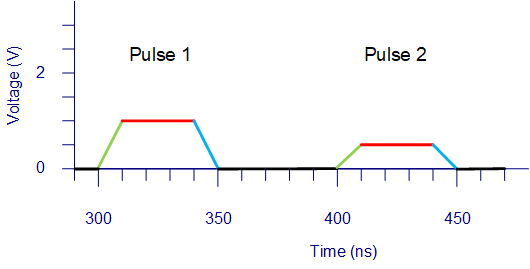
\includegraphics[width=0.7\linewidth]{figures/3.1.1.png}
%     \caption{Two pulses with pulse 2 having half the amplitude of pulse 1.}
%     \label{fig:gain_scale_example}
% \end{figure}

To fulfill the requirement to generate a pulse sequence, the pulse channel module uses Xilinx block RAM IPs, a state machine, and an interface to drive an external 16-bit DAC. One of the block RAMs is dedicated to the waveform table memory, where unique digital representations of pulses' waveforms are stored. A separate block RAM, known as the pulse definition table memory, holds configuration data for each pulse, including start time, sustain time, time and gain factors, waveform length, and a waveform identifier that links to the corresponding waveform stored in the waveform table memory. The state machine reads from both memories to select the appropriate waveform and configuration of a pulse, thereby driving the DAC to produce the desired pulse sequence. The area highlighted in purple in \autoref{fig:block_diagram} illustrates the relative placement of these two memories within the module, with further details discussed in later sections.

\begin{figure}[h]
    \centering
    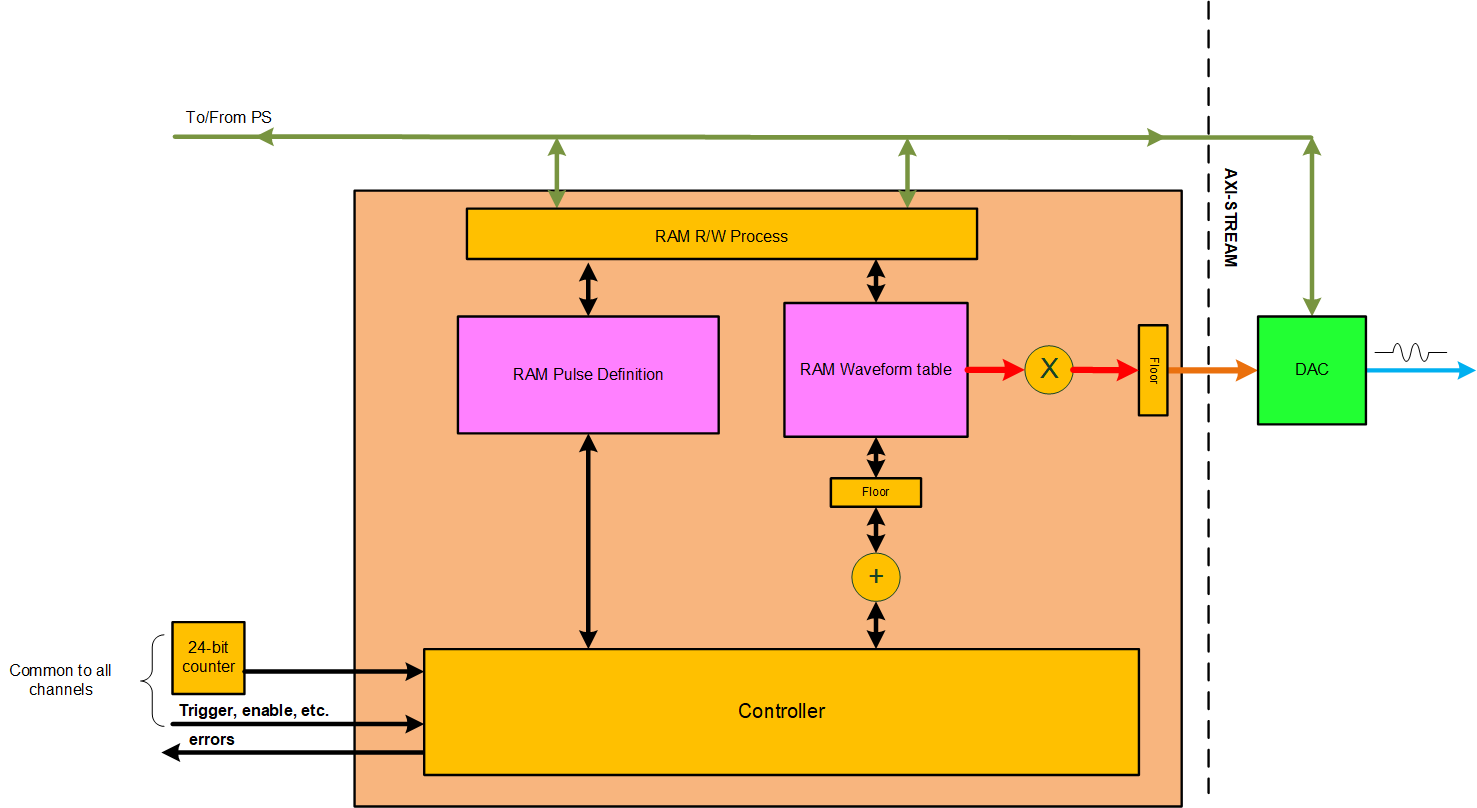
\includegraphics[width=1.0\linewidth]{figures/3.1.png}
    \caption{Block diagram of the pulse channel with two RAMs integrated.}
    \label{fig:block_diagram}
\end{figure}

All waveform data and parameters are loaded into memory via a word-addressable interface, as highlighted by the green arrow in \autoref{fig:block_diagram}. This interface supports both configuration and monitoring, allowing the module to select between the RAM blocks or perform real‐time diagnostics and debugging. The design enables rapid reconfiguration and continuous system oversight, which assists in maintaining high performance during pulse sequence generation.

Error handling is integrated into the module. Dedicated error signals are generated during pulse generation to detect anomalies and trigger immediate responses. Pipeline delays are carefully managed to ensure signal synchronization and maintain timing margins across the data path.

\section{Setup}
\subsubsection{Waveform Table}

\begin{figure}[htbp]
    \setlength{\abovecaptionskip}{5pt}    % Reduces space above caption
    \setlength{\belowcaptionskip}{5pt}    % Reduces space below caption
    \centering
    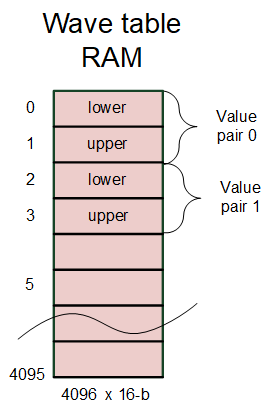
\includegraphics[width=0.55\linewidth]{figures/3.3.png}
    \caption{Memory layout for waveform table}
    \label{fig:wavetable}
\end{figure}
% The waveform table memory is designed to store 16-bit values that define the shape of the waveform for each pulse in a pulse sequence. The memory is a True Dual Port RAM created using Xilinx Block Memory Generator \cite{blockmemgen}. One of the ports is dedicated to user read and write values into the memory. The other port is read-only and used for the pulse channel's internal controller shown in the orange box at the bottom part of \autoref{fig:block_diagram}. Illustrated in \autoref{fig:wavetable}, user loads two 16-bit values for each memory write, while the internal controller uses one 16-bit value for each read access. While the controller performs read access to the memory, the user is also allowed to perform read access from a different port. This allows read-time monitoring and debug of the waveform values without interfering with the pulse generation. 

The waveform table memory stores 16-bit values that define each pulse's shape. It is implemented as a dual-port RAM using the Xilinx Block Memory Generator \cite{blockmemgen}. One port accepts user read and write operations, while the other, designated for the pulse channel's internal controller (highlighted in the orange box in \autoref{fig:block_diagram}), is read-only. As illustrated in \autoref{fig:wavetable}, users write two 16-bit values per memory access, while the controller reads one 16-bit value. This simultaneous access facilitates real-time monitoring and debugging of waveform values without interfering with pulse generation.



% The memory allocation of the waveform table memory is dynamic. User should specify in the pulse configuration the memory region should a pulse use for its waveform. The waveform table allows multiple pulse referencing the same memory region. This capability is beneficial when different pulses in a pulse sequence shares the same waveform features. This design is purpose-build to maximize memory utilization, ensuring each waveform receive space only what is necessary. 

In addition, the waveform table memory employs dynamic allocation. Each pulse configuration includes a start address and a waveform length, which together uniquely identify a waveform in memory. This design allows pulses with a common waveform to share the same memory region, ensuring that only the space required for these characteristics is allocated.

\subsection{Pulse Definition}

\begin{figure}[htbp]
    \setlength{\abovecaptionskip}{0pt}    % Reduces space above caption
    \setlength{\belowcaptionskip}{0pt}    % Reduces space below caption
    \centering
    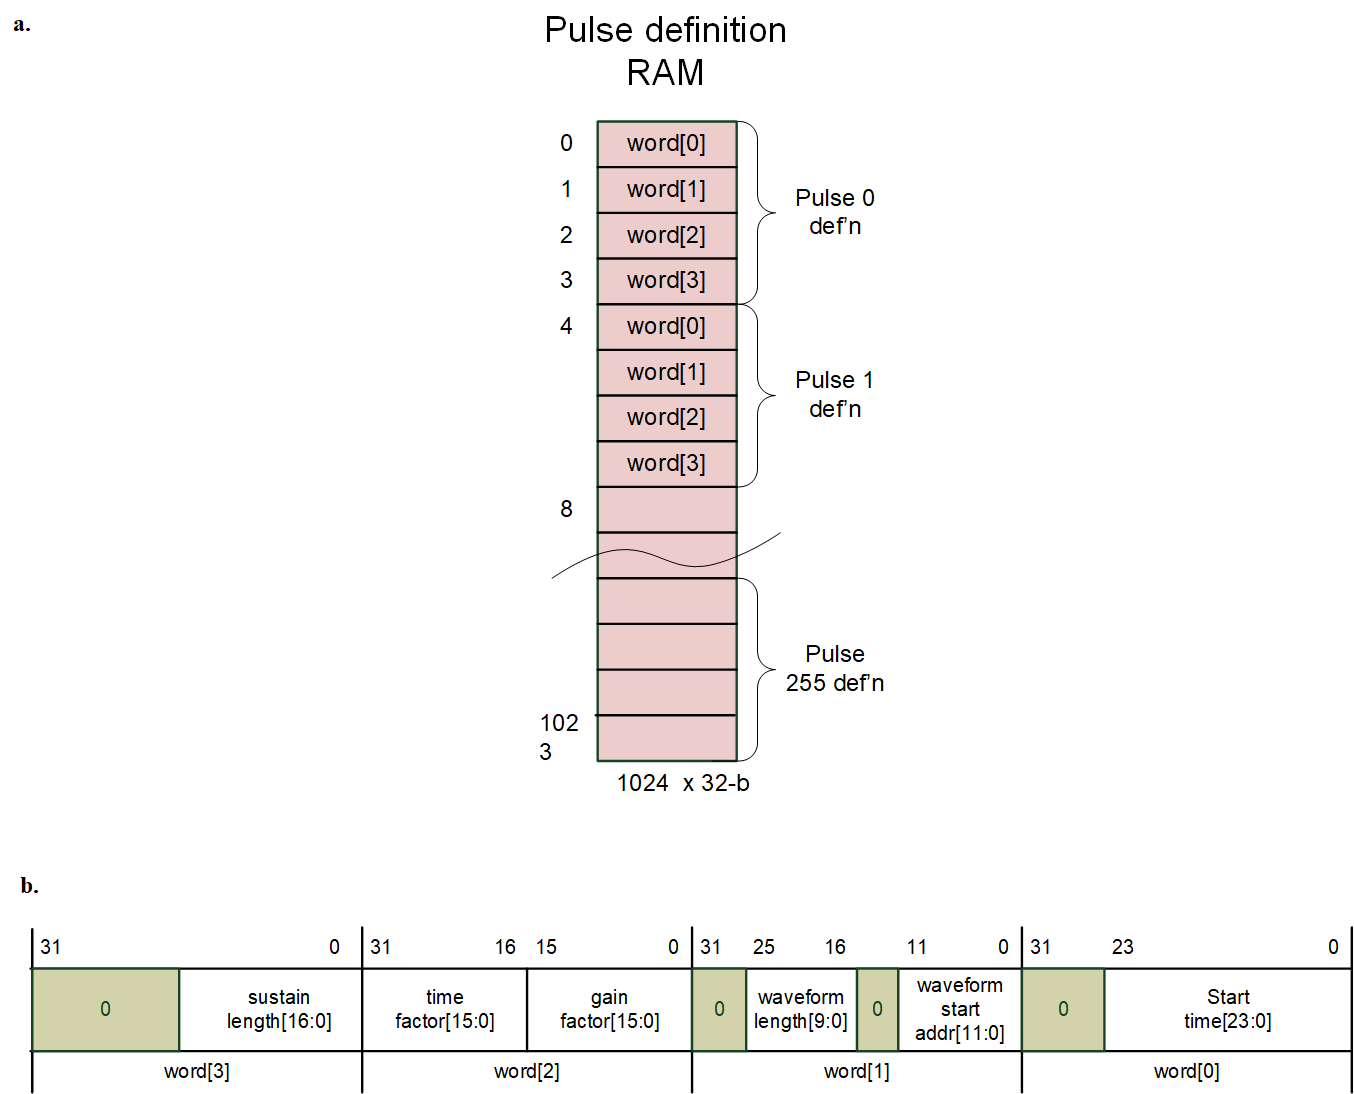
\includegraphics[width=1\linewidth]{figures/3.2.png}
    \caption{\centering{Pulse Definition RAM overall allocation. \textbf{a}, the overall allocation in the memory. \textbf{b}, specific bit-wise allocations of each pulse’s parameter.}}
    \label{fig:pd}
\end{figure}
% The pulse definition memory, similar to the waveform table memory, is a Xilinx Dual-Port RAM. Differing from the waveform table, the pulse definition employs a static addressing scheme, where each user-defined pulse configuration is placed into four consecutive 32-bit memory locations. This means that the configuration for each pulse stored sequentially, as illustrated in \autoref{fig:pd}a. In other words, each pulse configuration set is a 128-bit entry, occupying four consecutive word addresses. This structured approach ensured efficient storage and retrieval of each pulse's configurations. By organizing the memory in this manner, the system can handle significant numbers of pulses while maintaining clarity and ease of access. The allocation of each pulse a pulse's configuration for each entry is shown in \autoref{fig:pd}b.

The pulse definition memory, analogous to the waveform table memory, is implemented using a Xilinx Dual-Port RAM. Unlike the waveform table, it adopts a static allocation scheme, whereby each user-defined pulse configuration is assigned four consecutive 32-bit words, forming a 128-bit entry (see \autoref{fig:pd}a). This organized structure minimizes addressing overhead and simplifies data retrieval. Figure \autoref{fig:pd}b illustrates the specific allocation of each pulse configuration in the pulse definition memory.

\subsection{Internal Controller}

\begin{figure}[htbp]
    \setlength{\abovecaptionskip}{0pt}    % Reduces space above caption
    \setlength{\belowcaptionskip}{0pt}    % Reduces space below caption
    \centering
    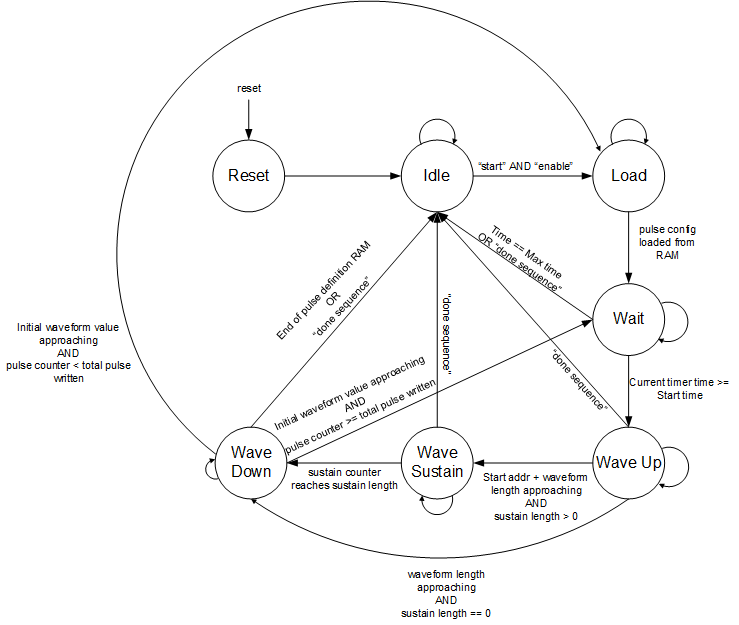
\includegraphics[width=1\linewidth]{figures/3.4.png}
    \caption{State Diagram of the Pulse Channel Module}
    \label{fig:fsm}
\end{figure}


The internal controllers of the Pulse Channel module generate a precise pulse sequence by transitioning through a series of well-defined states, as illustrated in \autoref{fig:fsm}. The module is activated when an external trigger is received and the module is enabled, as shown in the bottom left of \autoref{fig:block_diagram}. Upon activation, it loads the required data from the pulse definition memory into a set of registers and then enters a waiting state until the 24-bit timer reaches the predetermined start time. This design guarantees precise pulse generation at the intended moments, ensuring seamless system synchronization.

When the timer reaches the start time, the module moves sequentially through the rise, sustain, and fall stages. During these stages, it carefully shapes the pulse by controlling both the waveform table address and its data output using the time ("+" sign in \autoref{fig:block_diagram}) and gain ("x" sign in \autoref{fig:block_diagram}) factor values. After the fall stage, the module evaluates whether additional pulses remain in the pulse definition memory. If there are more pulses, it immediately loads the next one. Otherwise, it waits for a "done sequence" signal before going idle.

An internal pulse counter monitors the current entry in the pulse definition memory and increments each time a new pulse is loaded. Because each pulse definition spans four memory addresses, the counter increases by four with every update. Another counter tracks the number of clock cycles that the sustain phase has lasted following the rise stage. When this counter reaches the defined sustain length, the state machine transitions to the fall stage. This organized, stage-based design simplifies the control logic while enhancing timing precision and signal integrity. 

In parallel, a dedicated process manages memory read and write operations via the CPU interface, as indicated by the green arrows in \autoref{fig:block_diagram}. Through this interface, users designate the target memory by including the appropriate identifier in the provided address. For the waveform table, each write operation transfers a 32-bit value, which together constitute one entry. This arrangement yields a total of 2048 available entries for user write accesses. In contrast, each pulse definition entry spans four 32-bit words. Therefore, it takes four consecutive write operations to complete one pulse definition entry. This clear division of memory operations not only ensures efficient and reliable data transfer but also simplifies the addressing scheme, maintaining data integrity and responsiveness in real-time FPGA applications.

\section{Error Handling}

The pulse channel is engineered to be highly resilient, capable of handling both typical user inputs and unusual or invalid parameters. It accounts for common values as well as edge cases that might otherwise disrupt system operation. While the software interface manages most user-induced errors, the built-in error registers and handling mechanisms serve as the final safeguard. This layered approach prevents hazardous inputs from causing system failures, ensuring that the design remains safe and reliable even under unexpected conditions.

To ensure performance, several potential cases must be carefully considered. The design guarantees that pulses begin only when the current time meets or exceeds their scheduled start. Special attention is given to the sustain length. For instance, if a pulse definition specifies a flat-top length of zero, the system immediately transitions to the fall stage. The module also keeps track of the total number of generated pulses using the internal pulse counter, which helps maintain proper sequence control. Moreover, if the start time of a subsequent pulse is earlier than that of the previous one, the pulse is omitted to preserve timing integrity.

Additionally, the design manages cases where a waveform exceeds the capacity of the waveform table memory. In such instances, the system either wraps the addresses correctly back into the valid range or triggers an error flag in an 8-bit register, with each bit defined in \autoref{table:erro_regs}. 
% One-hot encoding ensures that the error register uniquely represents each error condition with a single active flag. 
When a specific error occurs, the system sets only the corresponding flag. This clear mapping simplifies fault diagnosis and reduces ambiguity during troubleshooting. When an error is detected, the system stops waveform generation to prevent the further propagation of invalid data, thereby maintaining overall system integrity. Furthermore, the registers are designed to log and maintain these error events, aiding in prompt debugging and corrective measures. The error registers can be cleared with an external clear flag or by resetting the system. Some registers have no error details assigned yet, allowing for future expandability based on further testing results.
\begin{table}[h]
\setlength{\abovecaptionskip}{5pt}    % Reduces space above caption
\setlength{\belowcaptionskip}{5pt}    % Reduces space below caption
\centering
\caption{Error Registers}
\label{table:erro_regs}
\begin{tabular}{|c|l|}
\hline
Register Bit & Error Details \\
\hline
0 & Wave table memory overflow \\
\hline
1 & Waveform size $\leq$ 1 (need minimum of 2 values) \\
\hline
2 & Time factor bigger than the size of the rise \\
\hline
3 & Gain factor $>$ 1 \\
\hline
4 & Time factor $<$ 1 \\
\hline
5 & Start time too early (minimum 50ns apart between pulses) \\
\hline
6 & \textit{Not yet assigned} \\
\hline
7 & \textit{Not yet assigned} \\
\hline
\end{tabular}
\end{table}